\documentclass[11pt,openany]{article}

\usepackage{mathtools, commath}
% Packages for formatting
\usepackage[margin=1in]{geometry}
\usepackage{fancyhdr}
\usepackage{enumerate}
\usepackage{graphicx}
\usepackage{kotex}
\usepackage{arydshln} % Include this package
\usepackage{bbding}
\usepackage{amsmath}
\usepackage{amsthm}
\usepackage[dvipsnames,table]{xcolor}
\usepackage{amssymb, amsfonts}
\usepackage{wasysym}
\usepackage{footnote}
\usepackage{tablefootnote}
\usepackage{arydshln} % Include this package
% Fonts
\usepackage[T1]{fontenc}
\usepackage[utf8]{inputenc}
\usepackage{newpxtext,newpxmath}
\usepackage{sectsty}

% Define colors
\definecolor{TealBlue1}{HTML}{0077c2}
\definecolor{TealBlue2}{HTML}{00a5e6}
\definecolor{TealBlue3}{HTML}{b3e0ff}
\definecolor{TealBlue4}{HTML}{00293c}
\definecolor{TealBlue5}{HTML}{e6f7ff}

\definecolor{thmcolor}{RGB}{231, 76, 60}
\definecolor{defcolor}{RGB}{52, 152, 219}
\definecolor{lemcolor}{RGB}{155, 89, 182}
\definecolor{corcolor}{RGB}{46, 204, 113}
\definecolor{procolor}{RGB}{241, 196, 15}

\usepackage{color,soul}
\usepackage{soul}
\newcommand{\mathcolorbox}[2]{\colorbox{#1}{$\displaystyle #2$}}
\usepackage{cancel}
\newcommand\crossout[3][black]{\renewcommand\CancelColor{\color{#1}}\cancelto{#2}{#3}}
\newcommand\ncrossout[2][black]{\renewcommand\CancelColor{\color{#1}}\cancel{#2}}

\usepackage{hyperref}
\usepackage{booktabs}

% Chapter formatting
\definecolor{titleTealBlue}{RGB}{0,53,128}
\usepackage{titlesec}
\titleformat{\section}
{\normalfont\sffamily\Large\bfseries\color{titleTealBlue!100!gray}}{\thesection}{1em}{}
\titleformat{\subsection}
{\normalfont\sffamily\large\bfseries\color{titleTealBlue!50!gray}}{\thesubsection}{1em}{}

%Tcolorbox
\usepackage[most]{tcolorbox}
\usepackage{multirow}
\usepackage{multicol}

\usepackage[linesnumbered,ruled]{algorithm2e}
\usepackage{algpseudocode}
\usepackage{setspace}
\SetKwComment{Comment}{/* }{ */}
\SetKwProg{Fn}{Function}{:}{end}
\SetKw{End}{end}
\SetKw{DownTo}{downto}

% Define a new environment for algorithms without line numbers
\newenvironment{algorithm2}[1][]{
	% Save the current state of the algorithm counter
	\newcounter{tempCounter}
	\setcounter{tempCounter}{\value{algocf}}
	% redefine the algorithm numbering (remove prefix)
	\renewcommand{\thealgocf}{}
	\begin{algorithm}
	}{
	\end{algorithm}
	% Restore the algorithm counter state
	\setcounter{algocf}{\value{tempCounter}}
}

\usepackage{adjustbox}
% Header and footer formatting
\pagestyle{fancy}
\fancyhead{}
\fancyhf{}
\rhead{\textcolor{TealBlue2}{\large\textbf{기대수(기초부터 대학원 수학까지 시리즈) 3기}}}%\rule{3cm}{0.4pt}}
\lhead{\textcolor{TealBlue2}{\large\textbf{수학의 즐거움, Enjoying Math}}}
% Define footer
%\newcommand{\footer}[1]{
%\begin{flushright}
%	\vspace{2em}
%	\includegraphics[width=2.5cm]{school_logo.jpg} \\
%	\vspace{1em}
%	\textcolor{TealBlue2}{\small\textbf{#1}}
%\end{flushright}
%}
%\rfoot{\large Department of Information Security, Cryptogrphy and Mathematics, Kookmin Uni.\includegraphics[height=1.5cm]{school_logo.jpg}}
\fancyfoot{}
\fancyfoot[C]{-\thepage-}

\usepackage{tcolorbox}
\tcbset{colback=white, arc=5pt}

\definecolor{axiomcolor}{HTML}{a88bfa}
\definecolor{defcolor}{RGB}{52, 152, 219}
\definecolor{procolor}{RGB}{241, 196, 15}
\definecolor{thmcolor}{RGB}{231, 76, 60}
\definecolor{lemcolor}{RGB}{155, 89, 182}
\definecolor{corcolor}{RGB}{46, 204, 113}
\definecolor{execolor}{RGB}{90, 128, 127}

% Define a new command for the custom tcolorbox
\newcommand{\axiombox}[2][]{%
	\begin{tcolorbox}[colframe=axiomcolor, title={\color{white}\bfseries #1}]
		#2
	\end{tcolorbox}
}

\newcommand{\defbox}[2][]{%
	\begin{tcolorbox}[colframe=defcolor, title={\color{white}\bfseries #1}]
		#2
	\end{tcolorbox}
}

\newcommand{\lembox}[2][]{%
	\begin{tcolorbox}[colframe=lemcolor, title={\color{white}\bfseries #1}]
		#2
	\end{tcolorbox}
}

\newcommand{\probox}[2][]{%
	\begin{tcolorbox}[colframe=procolor, title={\color{white}\bfseries #1}]
		#2
	\end{tcolorbox}
}

\newcommand{\thmbox}[2][]{%
	\begin{tcolorbox}[colframe=thmcolor, title={\color{white}\bfseries #1}]
		#2
	\end{tcolorbox}
}

\newcommand{\corbox}[2][]{%
	\begin{tcolorbox}[colframe=corcolor, title={\color{white}\bfseries #1}]
		#2
	\end{tcolorbox}
}



\usepackage{amsthm}

% Define custom theorem styles
\newtheoremstyle{dotless} % Name of the style
{3pt} % Space above
{3pt} % Space below
{\itshape} % Body font
{} % Indent amount
{\bfseries} % Theorem head font
{} % Punctuation after theorem head
{2.5mm} % Space after theorem head
{} % Theorem head spec

\newtheoremstyle{definitionstyle} % Name of the style
{3pt} % Space above
{3pt} % Space below
{} % Body font
{} % Indent amount
{\bfseries} % Theorem head font
{.} % Punctuation after theorem head
{2.5mm} % Space after theorem head
{} % Theorem head spec

% Applying custom styles
\theoremstyle{dotless}
\newtheorem{theorem}{Theorem} % Theorem environment with section-wise numbering
\newtheorem{proposition}[theorem]{Proposition} % Theorem environment with section-wise numbering
\newtheorem{lemma}[theorem]{Lemma} % Lemma shares the counter with theorem
\newtheorem{corollary}[theorem]{Corollary} % Corollary shares the counter with theorem

\theoremstyle{definitionstyle}
\newtheorem*{observation}{\textcolor{Magenta}{Observation}}
\newtheorem{definition}{Definition} % Definition shares the counter with theorem
\newtheorem{example}{Example} % Example shares the counter with theorem
\newtheorem{exercise}{Exercise} % Example shares the counter with theorem
\newtheorem{remark}{Remark} % Remark shares the counter with theorem
\newtheorem*{note}{Note}

\newtheorem*{definition*}{Definition} % Definition shares the counter with theorem
\newtheorem*{example*}{Example} % Example shares the counter with theorem
\newtheorem*{exercise*}{\textcolor{violet}{Exercise}} % Example shares the counter with theorem
\newtheorem*{remark*}{Remark} % Remark shares the counter with theorem


\usepackage{tikz}
\usepackage{tikz-cd}
\usepackage{tikz-3dplot}
\usepackage{pgfplots}
\pgfplotsset{compat=newest} % Adjust to your version of pgfplots
\def\Circlearrowleft{\ensuremath{%
		\rotatebox[origin=c]{180}{$\circlearrowleft$}}}
\def\Circlearrowright{\ensuremath{%
		\rotatebox[origin=c]{180}{$\circlearrowright$}}}
\def\CircleArrowleft{\ensuremath{%
		\reflectbox{\rotatebox[origin=c]{180}{$\circlearrowleft$}}}}
\def\CircleArrowright{\ensuremath{%
		\reflectbox{\rotatebox[origin=c]{180}{$\circlearrowright$}}}}
\usetikzlibrary{
	3d, % For 3D drawing
	angles,
	arrows,
	arrows.meta,
	backgrounds,
	bending,
	calc,
	decorations.pathmorphing,
	decorations.pathreplacing,
	decorations.markings,
	fit,
	matrix,
	patterns,
	patterns.meta,
	positioning,
	quotes,
	shadows,
	shapes,
	shapes.geometric,
	tikzmark
}
\tikzset{
	% single mid‐path arrow
	mid arrow/.style={
		decoration={
			markings,
			mark=at position 0.5 with {\arrow{Stealth[scale=1.2]}}
		},
		postaction={decorate},
	},
	% style for field arrows
	field arrow/.style={
		-{Stealth[scale=1.0]},
		thick,
		blue!70!black,
	},
}
\newcommand{\ie}{\textnormal{i.e.}}
\newcommand{\rsa}{\mathsf{RSA}}
\newcommand{\rsacrt}{\mathsf{RSA}\textendash\mathsf{CRT}}
\newcommand{\inv}[1]{#1^{-1}}

%New Command
%\newcommand{\set}[1]{\left\{#1\right\}}
\newcommand{\N}{\mathbb{N}}
\newcommand{\Z}{\mathbb{Z}}
\newcommand{\Q}{\mathbb{Q}}
\newcommand{\R}{\mathbb{R}}
\newcommand{\cR}{\mathcal{R}}
\newcommand{\C}{\mathbb{C}}
\newcommand{\F}{\mathbb{F}}
\newcommand{\nbhd}{\mathcal{N}}
\newcommand{\Log}{\operatorname{Log}}
\newcommand{\Arg}{\operatorname{Arg}}
\newcommand{\pv}{\operatorname{P.V.}}

\newcommand{\of}[1]{\left( #1 \right)} 
%\newcommand{\abs}[1]{\left\lvert #1 \right\rvert}
%\newcommand{\norm}[1]{\left\| #1 \right\|}

\newcommand{\sol}{\textcolor{magenta}{\bf Sol}}
\newcommand{\conjugate}[1]{\overline{#1}}

\newcommand{\res}{\operatorname{res}}
\DeclareMathOperator*{\Res}{\operatorname{Res}}

%\renewcommand{\Re}{\operatorname{Re}}
%\renewcommand{\Im}{\operatorname{Im}}

\newcommand{\cyclic}[1]{\langle #1 \rangle}
\newcommand{\uniform}{\overset{\$}{\leftarrow}}
\newcommand{\xmark}{\textcolor{red}{\XSolidBrush}}
\newcommand{\vmark}{\textcolor{green!75!black}{\CheckmarkBold}}

\newcommand{\gen}[1]{\langle #1 \rangle}
\newcommand{\Gen}[1]{\left\langle #1 \right\rangle}

\newcommand{\img}[1]{\text{Img}(#1)}
\newcommand{\Img}[1]{\text{Img}\left(#1\right)}
\newcommand{\preimg}[1]{\text{Img}^{-1}(#1)}
\newcommand{\Preimg}[1]{\text{Img}^{-1}\left(#1\right)}

\newcommand{\relation}{\mathrel{\mathcal{R}}}
\newcommand{\injection}{\rightarrowtail}
\newcommand{\surjection}{\twoheadrightarrow}
\newcommand{\id}{\textnormal{id}}

\newcommand{\eqclass}[1]{\left[#1\right]}

% Define custom colors for O and X
\newcommand{\yes}{\textcolor{blue}{\bf \fullmoon}}
\newcommand{\no}{\textcolor{red}{\bf \texttimes}}

\DeclarePairedDelimiter\ceil{\lceil}{\rceil}
\DeclarePairedDelimiter\floor{\lfloor}{\rfloor}
%\renewcommand{\floor}[#1]{\lfloor #1\rfloor}
%\newcommand{\Floor}[#1]{\left\lfloor #1\right\rfloor}
%\newcommand{\ceil}[#1]{\lceil #1\rceil}
%\newcommand{\Ceil}[#1]{\left\lceil #1\right\rceil}

\newcommand{\topology}{\mathscr{T}}
\newcommand{\sequence}[1]{\langle #1\rangle}

\setstretch{1.25}
\begin{document}
\pagenumbering{arabic}
\begin{center}
	\huge\textbf{Advanced Calculus I}\\
	\vspace{0.5em}
	\large{Ji, Yong-hyeon}\\
	\vspace{0.5em}
	\normalsize{\today}\\
\end{center}

\noindent We cover the following topics in this note.
\begin{itemize}
	\item Least Upper Bound Property (Completeness Axiom)
	\item Equivalence Relations
	\item Equivalence Classes
\end{itemize}
\hrule\vspace{12pt}
\thmbox[Intermediate Value Theorem]{\begin{theorem*}
	Let $[a,b]\subseteq\mathbb{R}$ be a real interval, and let $f:[a,b]\to\mathbb{R}$ be a continuous function on $[a,b]$. Let $f(a)<f(b)$. If $\gamma\in\mathbb{R}$ satisfies $f(a)<\gamma<f(b)$, then \[
	\exists c\in(a,b)\ \text{such that}\ f(c)=\gamma.
	\] \begin{center}
		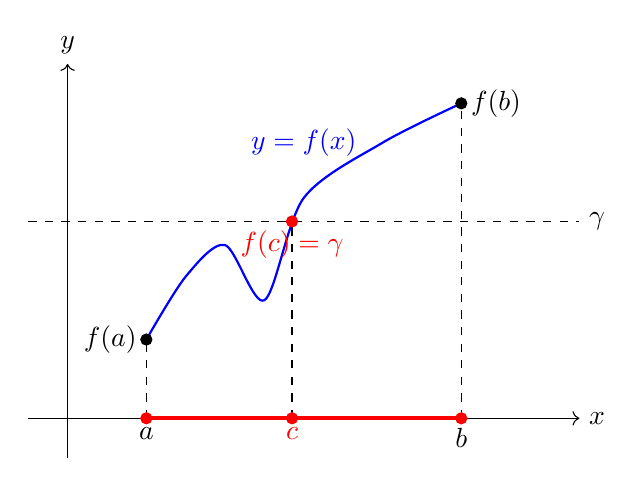
\begin{tikzpicture}[scale=1,domain=0:6,
	circledtail/.style={
		circle, draw, fill=white, inner sep=0pt, minimum size=6pt
	},
	open-open/.style={
		postaction={decorate, decoration={
				markings, 
				mark=at position 0 with {\node[circledtail]{};},  % Open circle at the start
				mark=at position 1 with {\node[circledtail]{};}   % Open circle at the end
		}}
	},
	closed-closed/.style={
		postaction={decorate, decoration={
				markings, 
				mark=at position 0 with {\filldraw[black] circle[radius=3pt];},  % Filled circle at start
				mark=at position 1 with {\filldraw[black] circle[radius=3pt];}   % Filled circle at end
		}}
	},
	open-closed/.style={
		postaction={decorate, decoration={
				markings, 
				mark=at position 0 with {\node[circledtail]{};},  % Open circle at the start
				mark=at position 1 with {\filldraw[black] circle[radius=3pt];}  % Filled circle at the end
		}},
		-{Stealth[scale=1.2]}
	},
	closed-open/.style={
		postaction={decorate, decoration={
				markings, 
				mark=at position 0 with {\filldraw[black] circle[radius=3pt];},  % Filled circle at the start
				mark=at position 1 with {\node[circledtail]{};}  % Open circle at the end
		}}
	}]
	% Draw the axes
	\draw[->] (-0.5,0) -- (6.5,0) node[right] {$x$};
	\draw[->] (0,-0.5) -- (0,4.5) node[above] {$y$};
	
	% Define points a and b on the x-axis
	\coordinate (A) at (1,0);
	\coordinate (B) at (5,0);
	
	% Define points f(a), f(b) and gamma
	\coordinate (FA) at (1,1); % f(a)
	\coordinate (FB) at (5,4); % f(b)
	\coordinate (GAMMA) at (0,2.5); % gamma horizontal line
	
	% Function graph
	\draw[color=blue,thick,smooth] plot coordinates {(1,1) (1.5,1.8) (2,2.2) (2.5,1.5) (3,2.8) (4,3.5) (5,4)};
	\node[blue] at (3,3.5) {$y=f(x)$};
		
	% Points on the graph
	\filldraw[black] (FA) circle (2pt) node[left] {$f(a)$};
	\filldraw[black] (FB) circle (2pt) node[right] {$f(b)$};
		
	% Draw vertical dashed lines for a and b
	\draw[dashed] (A) -- (FA);
	\draw[dashed] (B) -- (FB);
	
	% Labels for a and b
	\node[below] at (A) {$a$};
	\node[below] at (B) {$b$};
	
	\filldraw[red] (1,0) circle (2pt);
	\filldraw[red] (5,0) circle (2pt);
	\draw[red, line width=.5mm] (A) -- (B);
	
	% Gamma line and label
	\draw[dashed] (-0.5,2.5) -- (6.5,2.5) node[right] {$\gamma$};
	
	% Intersection point at c
	\draw[dashed] (2.85,0) -- (2.85,2.5);
	\filldraw[red] (2.85,2.5) circle (2pt) node[below] {$f(c) = \gamma$};
	\filldraw[red] (2.85,0) circle (2pt) node[below] {$c$};	
\end{tikzpicture}

	\end{center}
\end{theorem*}}
\begin{remark*}
\ \begin{center}
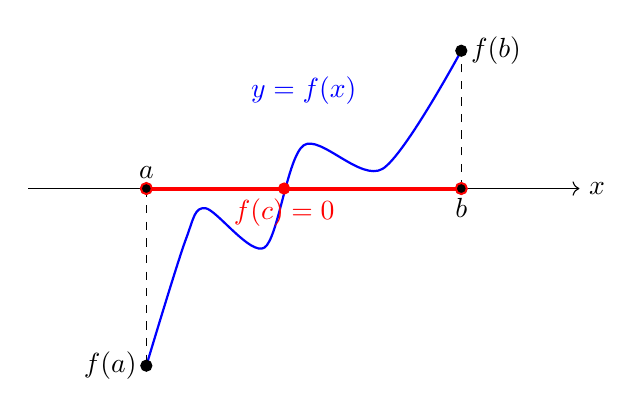
\begin{tikzpicture}[scale=1,domain=0:6]
	% Draw the axes
	\draw[->] (-0.5,-1.75) -- (6.5,-1.75) node[right] {$x$};
%	\draw[->] (0,-4) -- (0,0) node[above] {$f(x)$};
	
	% Define points a and b on the x-axis
	\coordinate (A) at (1,-1.75);
	\coordinate (B) at (5,-1.75);
	
	% Define points f(a), f(b) and gamma
	\coordinate (FA) at (1,-4); % f(a)
	\coordinate (FB) at (5,0); % f(b)
	\coordinate (GAMMA) at (0,2.5); % gamma horizontal line
	
	% Function graph
	\draw[color=blue,thick,smooth] plot coordinates {(1,-4) (1.5,-2.4) (1.75,-2) (2.5,-2.5) (3,-1.2) (4,-1.5) (5,0)};
	\node[blue] at (3,-.5) {$y=f(x)$};
	
	% Points on the graph
	\filldraw[black] (FA) circle (2pt) node[left] {$f(a)$};
	\filldraw[black] (FB) circle (2pt) node[right] {$f(b)$};
	
	% Draw vertical dashed lines for a and b
	\draw[dashed] (A) -- (FA);
	\draw[dashed] (B) -- (FB);
	
	% Labels for a and b
	\node[above] at (A) {$a$};
	\node[below] at (B) {$b$};
	
	\draw[red, line width=.5mm] (A) -- (B);
	\filldraw[black] (1,-1.75) circle (2pt);
	\filldraw[black] (5,-1.75) circle (2pt);
	
4	\draw[red, line width = .25mm] (1,-1.75) circle (2pt);
	\draw[red, line width = .25mm] (5,-1.75) circle (2pt);
	
	% Intersection point at c
	\filldraw[red] (2.75,-1.75) circle (2pt) node[below] {$f(c) = 0$};
\end{tikzpicture}

\end{center}
\end{remark*}

\begin{center}
	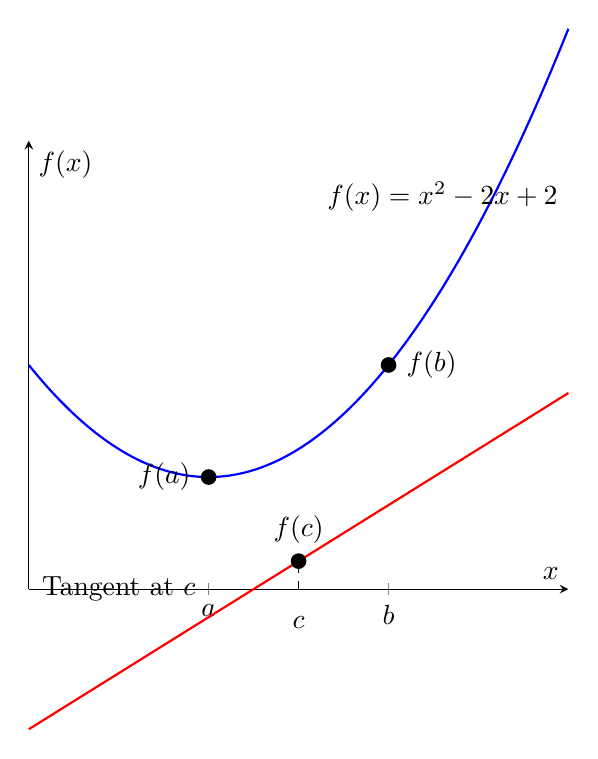
\begin{tikzpicture}
		\begin{axis}[
			axis lines = middle,
			xlabel = $x$,
			ylabel = {$f(x)$},
			xmin=0, xmax=3,
			ymin=0, ymax=4,
			xtick={1,2},
			xticklabels={$a$,$b$},
			ytick=\empty,
			clip=false,
			domain=0:3 % Set the domain for all plots
			]
			
			% Define the function f(x)
			\addplot[blue, thick, smooth, samples=100] {x^2 - 2*x + 2};
			\node at (axis cs:2.3,3.5) {$f(x) = x^2 - 2x + 2$};
			
			% Calculate derivative and define tangent line at c
			% c = 1.5, f'(c) = 2*(1.5) - 2 = 1
			% Tangent equation: y - f(c) = f'(c)(x - c)
			% f(c) = (1.5)^2 - 2*(1.5) + 2 = 0.25
			% y = 1*(x - 1.5) + 0.25 = x - 1.25
			\addplot[red, thick, domain=0:3] {x - 1.25};
			\node at (axis cs:0.5,0) {Tangent at $c$};
			
			% Points a, b, and c
			\node[label={180:{$f(a)$}},circle,fill,inner sep=2pt] at (axis cs:1,1) {};
			\node[label={0:{$f(b)$}},circle,fill,inner sep=2pt] at (axis cs:2,2) {};
			\node[label={90:{$f(c)$}},circle,fill,inner sep=2pt] at (axis cs:1.5,0.25) {};
			\draw[dashed, thin] (axis cs:1.5,0) -- (axis cs:1.5,0.25);
			\node at (axis cs:1.5, -0.3) {$c$};
			
		\end{axis}
	\end{tikzpicture}
\end{center}

%\begin{center}
%	\begin{tikzpicture}
%		\begin{axis}[
%			axis lines=middle,
%			xlabel=$x$,
%			ylabel={$f(x)$},
%			xmin=0, xmax=4,
%			ymin=-1, ymax=1,
%			xtick={1,3},
%			xticklabels={$a$,$b$},
%			ytick=\empty,
%			clip=false,
%			domain=0:4, % Set the domain for all plots
%			samples=100,
%			smooth
%			]
%			
%			% Define the function f(x)
%			\addplot[blue, thick] {x^2 - 4*x + 3}; % Polynomial f(x) = x^2 - 4x + 3
%			\node at (axis cs:3.5,0.5) {$f(x) = x^2 - 4x + 3$};
%			
%			% Point where f(x) = 0, solving the equation x^2 - 4x + 3 = 0
%			% Roots are at x = 1 (f(a)) and x = 3 (f(b)), f(c) = 0 at x = 2
%			\node[label={270:{$f(a)$}},circle,fill,inner sep=2pt] at (axis cs:1,0) {};
%			\node[label={270:{$f(b)$}},circle,fill,inner sep=2pt] at (axis cs:3,0) {};
%			\draw[dashed, thin] (axis cs:2,0.5) -- (axis cs:2,-1); % Line at c to show crossing point
%			\node at (axis cs:2, -1.2) {$c$};
%			
%		\end{axis}
%	\end{tikzpicture}
%\end{center}

\section*{Least Upper Bound Property}
\defbox[Bounded Above and Below]{\begin{definition*}
	Let $S\subseteq\R$. We say $S$ is bounded above (below) if \[
	\exists\beta\in\mathbb{R}\ \text{such that}\ x\leq\beta (x\geq\alpha)\ \text{for each}\ x\in S.
	\]
\end{definition*}}
\begin{remark}
	\ \begin{itemize}
		\item $S=\varnothing$ is possible.
		\item 
	\end{itemize}
\end{remark}

\begin{exercise*}
	Show that $A=\set{1-\frac{1}{n}:n\in\N}$ has an upper bound and a lower bound.

\end{exercise*}

\begin{exercise*}
	Show that $\N$ has a lower bound, but do not have the upper bound.
	
	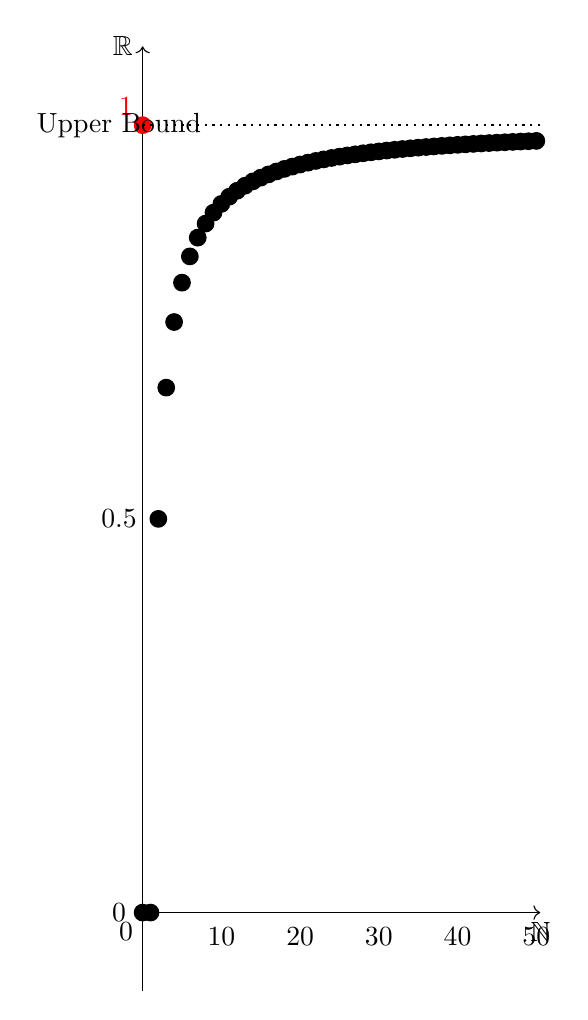
\begin{tikzpicture}[scale=10] % Scaling for better visualization
		
		% Draw axes
		\draw[->] (0, -0.1) -- (0, 1.1) node[left] {$\mathbb{R}$};  % y-axis
		\draw[->] (0, 0) -- (.505, 0) node[below] {$\mathbb{N}$};  % x-axis
		
		% Label for some x-axis values (representing natural numbers, scaled down)
		\foreach \n in {10, 20, 30, 40, 50} {
			\pgfmathsetmacro{\x}{\n/100} % Scaling the x-axis
			\node at (\x, -0.03) {\n};
		}
		
		% Plot points for n = 1, 2, ..., 100 with proper scaling
		\foreach \n in {1, 2, ..., 50} {
			\pgfmathsetmacro{\x}{\n/100}  % Scaling x-axis to fit 100 points
			\pgfmathsetmacro{\y}{1 - 1/\n} % y-axis corresponds to 1 - 1/n
			\filldraw[black] (\x, \y) circle (0.3pt);
		}
		
		% Mark lower bound at y = 0
		\filldraw[black] (0, 0) circle (0.3pt) node[below left] {$0$};
		
		% Mark upper bound at y = 1
		\filldraw[red] (0, 1) circle (0.3pt) node[above left] {$1$};
		
		% Dotted line to show the upper bound being approached but not reached
		\draw[dotted, thick] (0, 1) -- (.505, 1);
		
		% Label for upper bound
		\node at (-0.03, 1) {Upper Bound};
		
		% Label for some y-axis values
		\node at (-0.03, 0.5) {0.5};
		\node at (-0.03, 0) {0};
		
	\end{tikzpicture}
\end{exercise*}

\begin{exercise*}
	$B=\set{r\in\Q:r>0\land r^2<2}$. Then $B$ has a lower bound $\alpha=0$ but $B$ does not have the maximum element. To show it, it is enough to show if $p\in B$, then $\exists q\in B$ s.t. $p<q$.
	Take any $p\in B$. Take \[
	q=p+\frac{2-p^2}{p+2}>P.
	\] Then $q\in Q$ because $Q$ is a field.
\end{exercise*}

\axiombox[Least Upper Bound Property (Completeness Axiom)]{\begin{axiom*}
	
\end{axiom*}}


\begin{thebibliography}{9}
	\bibitem{advanced_calc_a}
	수학의 즐거움, Enjoying Math. ``수학 공부, 기초부터 대학원 수학까지, 4. 해석학 개론 (a) 완비성 공리.'' YouTube Video, 32:20. Published 
	September 09, 2019. URL: \url{https://www.youtube.com/watch?v=pHIImTBdBRs}.
\end{thebibliography}

\end{document}
